\documentclass[a4paper,12pt]{article}
\usepackage[utf8]{inputenc}
\usepackage[french]{babel}
\usepackage[T1]{fontenc}
\usepackage[top=2cm,bottom=2cm,left=2cm,right=2cm]{geometry}
\usepackage{graphicx}
\usepackage{wrapfig}
\usepackage{url}

\begin{document}

\begin{titlepage}
	\begin{center}
		\Large{Année universitaire 2016-2017}\\
		\Large{Université de Caen Basse-Normandie}\\[1cm]
		
		\huge{Rapport sur les raccourcis}\\
		\vspace{3cm}
			
		Emma Mauger - 21501058\\
		
	\normalsize{\textit{ ~ L2 Informatique}}\\
		\medskip
		\vspace{2cm}
		
	\end{center}
\end{titlepage}

\tableofcontents
\newpage

Dans le menu de notre IDE, vous avez pu remarquer qu'à côté de certaines options, il y avait des raccourcis que nous avions choisis en fonction de ce qui nous semblait être le mieux. Mais ces choix étaient personnels, et tous les membres du groupe n'approuvant pas certains choix, nous avons décidé de les rendre personnalisables.

\section{Réalisation}

\subsection{Partie interface}

Nous avons trois menus dans lesquels il y a des raccourcis. Ainsi, nous avons décidé de créer un fichier "racc\_defaut.json" qui contient un dictionnaire ayant pour clefs le noms de ces trois menus, et comme valeurs d'autres dictionnaires qui ont pour clefs les noms des fonctionnalités et comme valeurs une chaîne de caractères représentant le raccourci.

\begin{center}
	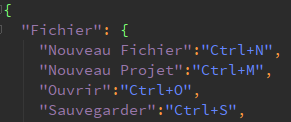
\includegraphics[scale=0.5]{images/ex_1.png}\\
	Ici, un aperçu du fichier "racc\_defaut.json".
\end{center}

Nous pouvons donc conserver tous les raccourcis de base et en proposer dès le lancement de l'IDE, au lieu de forcer l'utilisateur à en définir. Il peut donc choisir, via le menu "Fichier", dans le sous-menu "Paramètres", l'option Raccourcis, qui modifiera le fichier "racc\_utilisateur.json" créé lors du lancement de l'IDE si celui-ci n'existait pas déjà.

Cliquer sur cette option lui ouvrira une nouvelle fenêtre (une QDialog), dans laquelle trois onglets (des QTabWidget) seront disponibles. Ces trois onglets correspondent aux trois menus qui contiennent des raccourcis. Dans ces onglets, des lignes de saisies (des QLineEdit) seront apparentes permettront à l'utilisateur de rentrer ses propres raccourcis. Nous avons mis les raccourcis de base en fond pour que l'utilisateur ait un modèle. Cette interface est complétée par deux boutons, l'un qui valide les raccourcis et l'autre qui les remet à zéro, c'est-à-dire qu'il modifie les valeurs contenues dans le fichier "racc\_utilisateur.json",  et les remplace par les valeurs contenues dans le fichier "racc\_defaut.json".

\begin{center}
	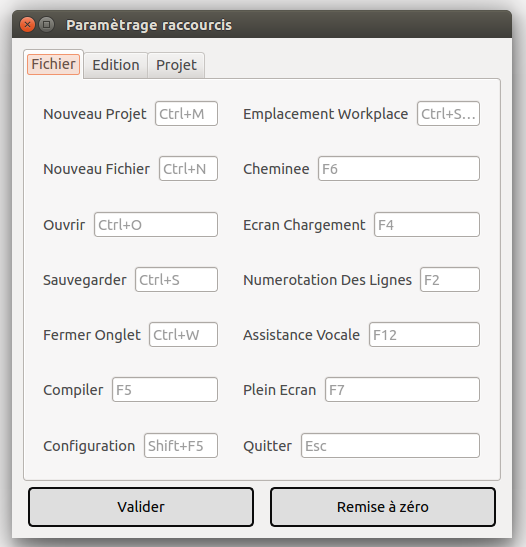
\includegraphics[scale=0.4]{images/ex_2.png}\\
	Un aperçu de la fenêtre permettant la modification des raccourcis.
\end{center}

\subsection{Partie modification}

En ce qui concerne la modification des raccourcis, il est possible de d'écrire tout ce que l'on veut dans les lignes de saisies. C'est lorsque l'on clique sur le bouton valider que la fonction qui valide un raccourci va être appelée. Ainsi, certaines combinaisons de touches ne sont pas permises, telles que "M+Shift+Ctrl". Nous avons aussi décidé de faire en sorte que si l'utilisateur écrit quelque chose de ce style : "Ctrl+Shift+JHGFFUTRF", on écrive dans le fichier "racc\_utilisateur.json" : "Ctrl+Shift+J".

\end{document}